%----------------------------------------------------------------------------------------
%   PACKAGES AND THEMES
%----------------------------------------------------------------------------------------

\documentclass{beamer}

\mode<presentation> {

% The Beamer class comes with a number of default slide themes
% which change the colors and layouts of slides. Below this is a list
% of all the themes, uncomment each in turn to see what they look like.

%\usetheme{default}
%\usetheme{AnnArbor}
%\usetheme{Antibes}
%\usetheme{Bergen}
%\usetheme{Berkeley}
%\usetheme{Berlin}
%\usetheme{Boadilla}
%\usetheme{CambridgeUS}
%\usetheme{Copenhagen}
%\usetheme{Darmstadt}
%\usetheme{Dresden}
%\usetheme{Frankfurt}
%\usetheme{Goettingen}
%\usetheme{Hannover}
%\usetheme{Ilmenau}
%\usetheme{JuanLesPins}
%\usetheme{Luebeck}
%\usetheme{Madrid}
%\usetheme{Malmoe}
%\usetheme{Marburg}
%\usetheme{Montpellier}
%\usetheme{PaloAlto}
%\usetheme{Pittsburgh}
%\usetheme{Rochester}
%\usetheme{Singapore}
\usetheme{Szeged}
%\usetheme{Warsaw}

% As well as themes, the Beamer class has a number of color themes
% for any slide theme. Uncomment each of these in turn to see how it
% changes the colors of your current slide theme.

%\usecolortheme{albatross}
%\usecolortheme{beaver}
%\usecolortheme{beetle}
%\usecolortheme{crane}
\usecolortheme{dolphin}
%\usecolortheme{dove}
%\usecolortheme{fly}
%\usecolortheme{lily}
%\usecolortheme{orchid}
%\usecolortheme{rose}
%\usecolortheme{seagull}
%\usecolortheme{seahorse}
%\usecolortheme{whale}
%\usecolortheme{wolverine}

%\setbeamertemplate{footline} % To remove the footer line in all slides uncomment this line
%\setbeamertemplate{footline}[page number] % To replace the footer line in all slides with a simple slide count uncomment this line

%\setbeamertemplate{navigation symbols}{} % To remove the navigation symbols from the bottom of all slides uncomment this line
}
\usepackage{minted}
\usepackage{graphicx} % Allows including images
\usepackage{booktabs} % Allows the use of \toprule, \midrule and \bottomrule in tables

%----------------------------------------------------------------------------------------
%   TITLE PAGE
%----------------------------------------------------------------------------------------

\title[OB+NMC - lolosk, charapod]{OpenBazaar and Namecoin Integration} % The short title appears at the bottom of every slide, the full title is only on the title page

\author{Kostis Lolos \\ Chara Podimata} % Your name
\institute[NTUA] % Your institution as it will appear on the bottom of every slide, may be shorthand to save space
{
National Technical University of Athens \\ % Your institution for the title page
\medskip
\textit{lolos.kostis@gmail.com \\ charapod@gmail.com} % Your email address
}
\date{\today} % Date, can be changed to a custom date

\begin{document}

\begin{frame}
\titlepage % Print the title page as the first slide
\end{frame}

\begin{frame}
\frametitle{Overview} % Table of contents slide, comment this block out to remove it
\tableofcontents % Throughout your presentation, if you choose to use \section{} and \subsection{} commands, these will automatically be printed on this slide as an overview of your presentation
\end{frame}

%----------------------------------------------------------------------------------------
%   PRESENTATION SLIDES
%----------------------------------------------------------------------------------------

%------------------------------------------------
\section{Bitcoin} 
%------------------------------------------------
\subsection{What is it}
\begin{frame}
\frametitle{Bitcoin: A new kind of currency}
\begin{itemize}
\item Proposed by Satoshi Nakamoto in 2008
\item Open Source implementation in 2009
\item \$10 Billion total value of coins in 2014
\item Decentralized
\item No central authority or control
\item Potentially Anonymous
\item Extremely low transaction fees
\end{itemize}
\end{frame}
%-----------------------------------------------
\subsection{How it works}
\begin{frame}
\frametitle{Bitcoin: A new kind of currency}
\begin{figure}[H]
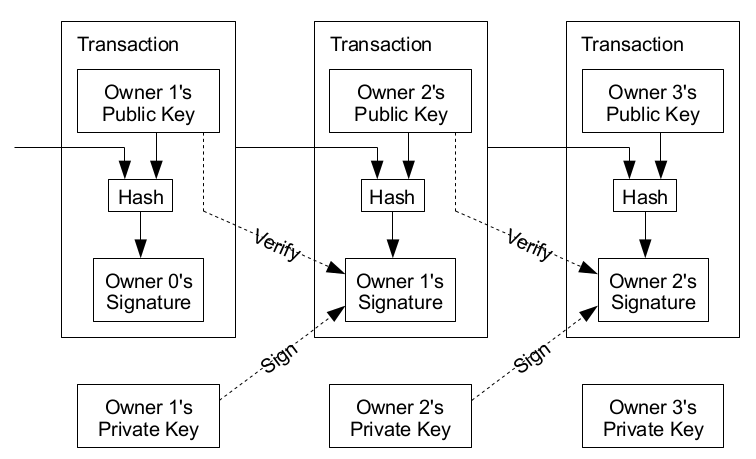
\includegraphics[width=0.6\textwidth]{screenshots/bitcoin.png}
\end{figure}
\begin{itemize}
\item Series of signatures \pause
\item Transactions stored in a block chain
\item Proof-of-work to prevent changes
\end{itemize}
\end{frame}
%-----------------------------------------------
\section{Namecoin}
%-----------------------------------------------
\subsection{Differences from Bitcoin}
\begin{frame}
\frametitle{Namecoin: A child of Bitcoin}
\begin{itemize}
\item The first fork of Bitcoin \pause
\item Names represented as special coins
\item Data associated with them \pause
\item Distributed DNS (.bit)
\end{itemize}
\end{frame}
%------------------------------------------------
\section{OpenBazaar}
%-------------------------------------------------
\subsection{What is OpenBazaar?}
%----------------------------------------------
\begin{frame}
\begin{figure}[H]
\centering
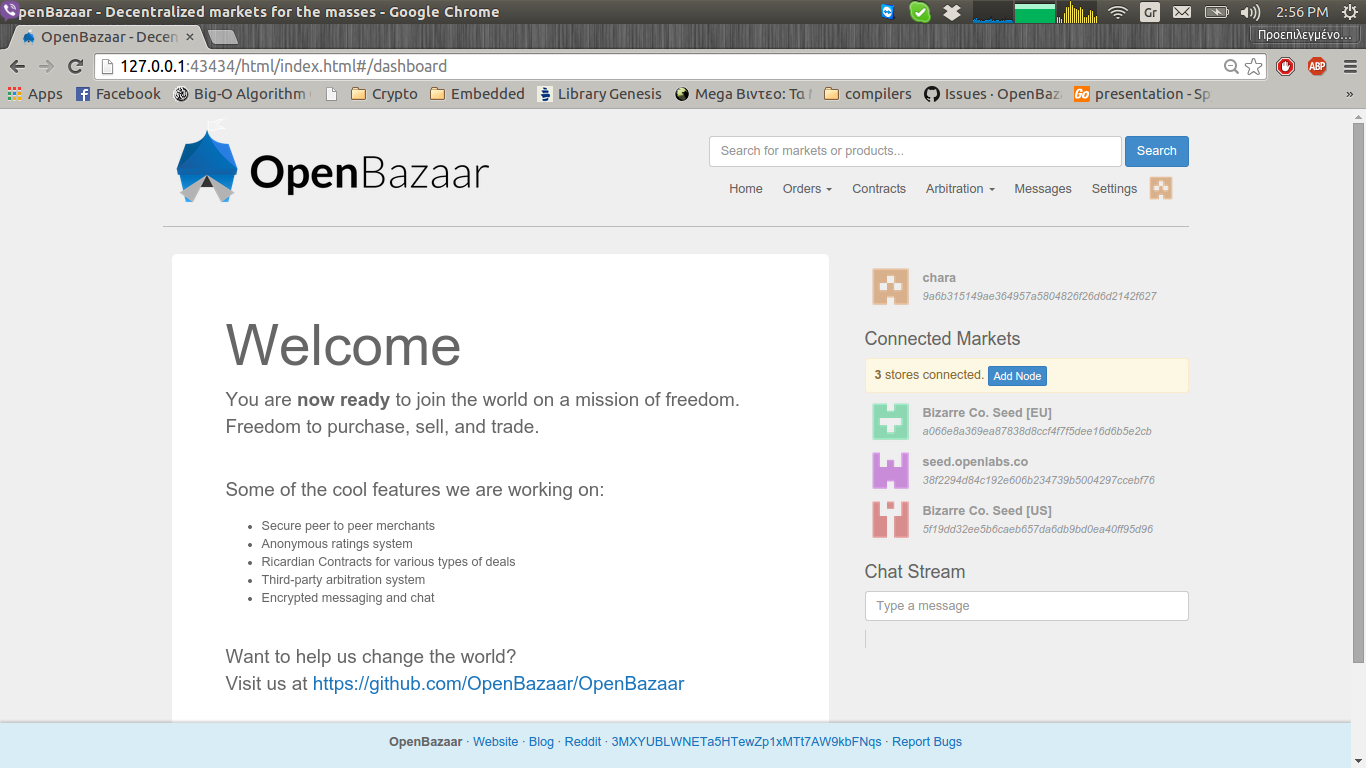
\includegraphics[width=1.00\textwidth]{screenshots/OB1.png}
\caption{Homepage}
\end{figure}
\end{frame}
%-------------------------------------------------
\begin{frame}
\frametitle{General Info} \pause
\begin{figure}[H]

\includegraphics[width=0.50\textwidth]{screenshots/OBlarge.png}
\end{figure}

\begin{itemize}
\item open-source project for a decentralized marketplace using BTC

\item {\bf no fees, no censorship}

\item p2p

\item OB = eBay + BitTorrent

\end{itemize}
\end{frame}
%---------------------------------------------------
\begin{frame}
\frametitle{Up to now online commerce means}
\begin{itemize}
\item centralized services \pause

\item restrictive policies\pause

\item fees for listing/selling goods\pause

\item only forms of payment accepted: credit cards, PayPal\pause

\item personal info required $\Rightarrow$ this info can be stolen or sold\pause

\item $\exists$ censorship
\end{itemize}\pause
OB puts back the power to users! No more users through a centralized service! We are directly connected, not censored, not charged!
\end{frame}
%---------------------------------------------------
\subsection{How does OB work}
\begin{frame}
Let's say you 've decided to sell your old laptop
\begin{itemize}
\item create a listing with product details + price and publish it on the network $\Rightarrow$ it now appears when keywords are searched
\item Prominent buyer can either accept your price or offer a new one
\item Once you have agreed on the price $\Rightarrow$ sign a contract with {\bf digital signatures}
\item contract sent to a third party (notaries, arbiters) $\Rightarrow$ she witnesses contract so as to release BTC
\end{itemize}

\end{frame}
%-------------------------------------------------
\begin{frame}
\frametitle{What if something goes wrong?}
People are no angels. Sellers may ship products in poorer condition or not ship products at all. \pause

{\bf What can we do about that?} \pause Third party! 

{\bf Remember!} BTC is released after  $2$ of $3$ parties agree

{\bf Ok, but how can I trust the third party?} \pause OB: {\bf reputation + rating system!}

$\Rightarrow$ users are allowed to rate (give feedback) about other users

$\Rightarrow$ scam a user $\rightarrow$ your reputation will suffer

$\Rightarrow$ when you are about to select a third party, pick one that the network trusts
\end{frame}
%----------------------------------------------
\subsection{Proof-of-burn and Reputation Pledges}
%-------------------------------------------
\begin{frame}
\frametitle{Proof-of-burn}
\begin{block}{Proof-of-burn}
Term used to describe the intentional and provable destruction of BTC for a particular purpose. Funds are intentionally sent to an address that is unspendable, meaning {\bf those coins are gone forever}.
\end{block} \pause

{\bf Ok, but why would anyone destroy BTC on purpose?} \pause
\begin{enumerate}
\item Past: to bootstrap one cryptocurrency from another (people burning coins in exchange for the new currency)

\item $\dots$ proof-of-burn as reputation pledges (OB)
\end{enumerate}
\end{frame}
%--------------------------------------------------
\begin{frame}
\frametitle{Reputation Pledges}
\begin{itemize}
\item users in OB are anonymous \pause $\Rightarrow$ sometimes difficult to determine whether they are trustworthy or not
\item {\bf Reputation System}: \pause helps you know which users have acted honestly in the past, and which haven't

\item For example, let's think of travelling salesmen $\dots$

\item Similarly in OB: You 've invested resources that create an incentive to keep a good reputation and impose significant cost for abandoning that reputation.
\end{itemize}
\end{frame}
%------------------------------------------------
\section{OB and Namecoin}
\subsection{Why OB and Namecoin}
\begin{frame}
\frametitle{Why OB and Namecoin}
\begin{itemize}
\item Human-readable address names \pause
\begin{itemize}
\item Users declare their Namecoin from the UI
\item Claimed Namecoin is relayed to other users
\item Namecoin is displayed as the unique Store URL \pause
\end{itemize}
\item Security \pause
\begin{itemize}
\item Each user: EC key $\Rightarrow$ GUID 
\item GUIDs stored in the blockchain 
\item Namecoin owner's GUID is matched with sender's GUID \pause
\item $\Rightarrow$ remote node is verified to be the Namecoin owner \pause
\item $\Rightarrow$ messages verified to be composed and encrypted by the same person
\end{itemize}
\end{itemize}
\end{frame}
%--------------------------------------------------
\begin{frame}
\begin{figure}[H]
\centering

\includegraphics[width=1.00\textwidth]{screenshots/Thanks.jpg}
\end{figure}
\end{frame}

\end{document}
